\chapter{Methodologie}
Dit hoofdstuk beschrijft de implementatie van ons systeem. Een eerste sectie handelt over een bestaande implementatie, waarop ons systeem is gebaseerd. Een tweede sectie beschrijft onze eigen extensie van de code van Karpathy, meer specifiek hoe we LDA topic verdelingen gebruiken om extra semantische informatie toe te voegen. Een derde sectie gaat over onze implementatie van het eerder vernoemde gLSTM netwerk zoals voorgesteld door Jia \todo{reference?}. De laatste sectie beschrijft hoe wij een normalisatie hebben toegevoegd aan de beam search om zinnen te maken (zoals voorgesteld door Jia \todo{ref}).

\section{Startpunt Karpathy} \todo{Betere titel}
Het startpunt van onze implementatie is de code aangereikt door A. Karpathy op zijn github pagina. Die bevat een implementatie van het recurrente neurale netwerk beschreven in \todo{reference naar karpathy}, alsook een implementatie die gebaseerd is op \todo{reference vinyals}. Op basis hiervan hebben wij een aantal extensies ge\"implementeerd.
\subsection{Recurrent Neuraal Netwerk}
Een eerste implementatie waarvan we zijn vertrokken is beschreven in Karpathy\todo{ref!}. Hij beschrijft een systeem dat op basis van een afbeelding een beschrijvende zin genereert. Dit gebeurt in twee stappen. Eerst wordt de afbeelding door middel van een CNN omgezet naar een vector representatie. Deze vector dient vervolgens als input voor een recurrent neuraal netwerk dat een grammaticaal correcte beschrijving genereert.

\paragraph{Afbeeldingsrepresentatie}
Het dataformaat van een afbeelding (2D matrix met een RGB waarde voor elke pixel) is onpraktisch om te gebruiken in neurale netwerken, aangezien die gebruik maken van gevectoriseerde input. Er is dus nood aan een vectorrepresentatie van de gebruikte afbeeldingen. De meeste bestudeerde algoritmes maken hiervoor gebruik van een convolutioneel neuraal netwerk. Het CNN dat momenteel het beste presteert is VGGNet, zoals beschreven in \todo{ref VGGNet}. Dit netwerk maakt gebruik van 16 layers, bestaande uit groepen van convolutionele layers afgewisseld met max-pool layers. De laatste layers van het netwerk zijn standaard (volledig verbonden) layers, gevolgd door een softmax layer, zoals te zien op figuur\ref{fig:vggnet}.

\begin{figure}[tb]
    \centering
    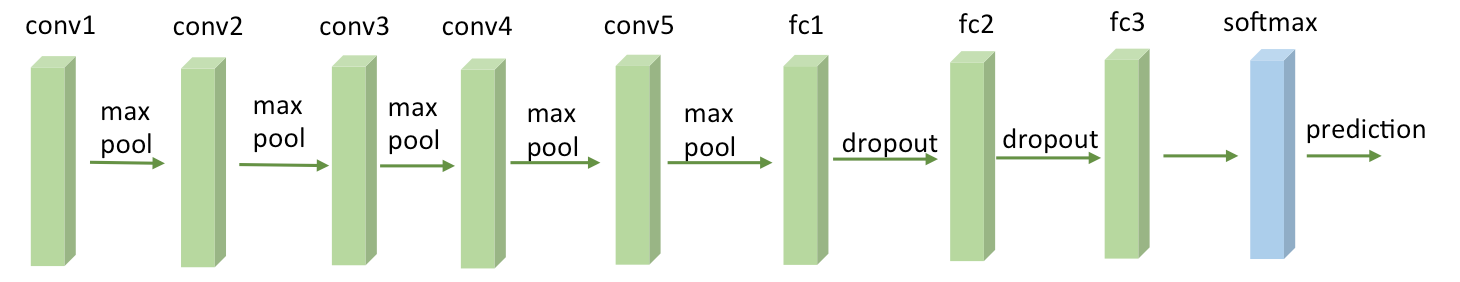
\includegraphics[width=\linewidth]{Images/vgg16.PNG}
    \caption{Globale structuur VGGNet met 16 layers}
    \label{fig:vggnet}
\end{figure}

De representatie die wordt gebruik door Karpathy is het resultaat van het netwerk voor de softmax layer wordt toegepast. Dit leidt tot een 4096-dimensionele vector, waarbij elke dimensie kan worden gezien als een bepaald concept dat al dan niet aanwezig is in de afbeelding. Deze dimensionaliteit is dezelfde voor alle afbeeldingen, als gevolg van een herschaling van de afbeeldingen tot een 512 op 512 pixel formaat vooraleer de vector wordt berekend.

VGGNet is momenteel het best presterende CNN voor afbeeldingsrepresentatie. Wij gebruiken in ons systeem dan ook de afbeeldingsvectors die berekend zijn met VGGNet. De gebruikte implementatie komt van Caffe \todo{Reference Caffe}.

\paragraph{Van afbeelding naar beschrijving}
De berekende vector representatie van de afbeelding dient als input voor een recurrent neuraal netwerk. Tijdens de training van het netwerk wordt op basis van de afbeelding, in combinatie met een speciale startvector die het begin van een zin aangeeft, het eerste woord voorspeld. Daarna wordt op basis van het eerste woord van de zin een voorspelling gemaakt voor het tweede woord. Dit proces herhaalt zich tot het einde van de zin bereikt is. Terugpropagatie op basis van stochastic gradient descent zorgt voor de juiste wijzigingen aan de gewichten van het netwerk. Een eenvoudige weergave van hoe het RNN een beschrijving genereert is te zien op figuur \ref{fig:rnntraining}.

\begin{figure}[tb]
    \centering
    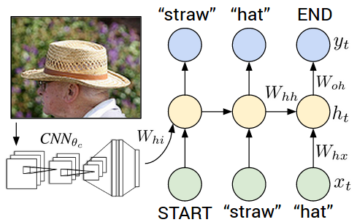
\includegraphics[width=0.5\linewidth]{Images/karpathy.PNG}
    \caption{Generatie van caption met recurrent neuraal netwerk}
\label{fig:rnntraining}
\end{figure}

Het genereren van captions gebeurt op basis van beam search. Hierbij wordt op basis van de afbeelding een ranking gemaakt van de meest waarschijnlijke eerste woorden voor de zin. De eerste $n$ woorden dienen dan als startpunt van de voorspelling van het tweede woord. Over alle mogelijke sets van twee woorden wordt opnieuw een rangschikking gemaakt, waarvan de $n$ beste resultaten worden bijgehouden. Dit proces herhaalt zich tot elke vertakking van de zoekboom is onderzocht, waarna de beste gegenereerde zin wordt gebruikt als eindresultaat.

\subsection{Long Short Term Memory Netwerk}

\section{Latent Dirichlet Analysis}
Het gebruik van Latent Dirichlet Analysis op een set van afbeeldingen en beschrijvingen heeft een groot voordeel in de taak van het genereren van nieuwe beschrijvingen. Deze sectie beschrijft welk proces wij hebben gevolgd om op basis van LDA extra semantische informatie te verkrijgen om te verwerken in onze implementatie en hoe de evaluatie van dit proces verliep.

\subsubsection{Berekening van topicverdeling}
\label{subs:Berekening van topicverdeling}
Het leren van het gebruikte LDA model gebeurt op een aangepaste versie van de Flickr30k dataset. De vijf captions worden gecombineerd tot \'e\'en zin, waarna stopwoorden worden verwijderd en de woorden door een Porter stemmer\todo{reference naar porter stemmer ?} worden gestemd. Deze zinnen worden dan gebruikt als input voor het algoritme. De afbeeldingen worden niet gebruikt, omdat er enkel op basis van tekst wordt gewerkt. Het doel is om op basis van een zin te kunnen bepalen welke topics het sterkst aanwezig zijn. Het idee hierachter is dat een topicverdeling ervoor kan zorgen dat het systeem woorden genereert die binnen het juiste topic passen.

Vervolgens begint het trainingsproces. Het aantal topics waarmee het systeem getraind wordt is variabel, en een schatting van het optimale aantal wordt gemaakt op basis van manuele evaluatie, zoals beschreven in sectie \ref{subs:Evaluatie}. Op basis van de zinnen uit de trainingsset berekent het algoritme de topic-woord verdelingen en de sentence-topic verdelingen. Dit model dient dan als transformatie voor de zinnen uit de test- en validatieset. De ``ground truth'' waarden van de sentence-topic verdelingen voor test- en validatieset worden berekend en opgeslagen.

Bij input van een nieuwe, ongeziene afbeelding moet het systeem in staat zijn om een topicverdeling af te leiden. Daarom is er een link nodig tussen een afbeeldingsrepresentatie en een topicverdeling. Hiervoor gebruiken we een simpel perceptron. Op basis van de eerder berekende ``ground truth'' waarden voor de test- en validatieset leert dit perceptron een mapping van afbeeldingsvector naar topicverdeling. Door middel van terugpropagatie worden de gewichten aangepast. Een vergelijking van negatieve logwaarschijnlijkheid leidt tot een optimalisatie van het aantal hidden layers en van de trainingstijd van het netwerk. Dit netwerk kan dan op het moment van testing zeer snel bepalen welke topicverdeling bij de afbeelding hoort. 

\subsubsection{Evaluatie}
\label{subs:Evaluatie}
De correctheid van de berekende topicverdelingen is uiteraard een kritiek punt in de performantie van ons systeem. Daarom hebben we manueel twee testen uitgevoerd. Een eerste test gaat over de optimalisatie van het aantal gebruikte topics. Bij de tweede test controleren we of de topicverdelingen die voorspeld worden door het perceptron wel passen bij de gegeven afbeelding.

Het optimaliseren van het aantal topics gebeurt op basis van manuele analyse van de woorden die voorkomen in elk topic. Op basis van de tien meest voorkomende woorden per topic proberen we een overkoepelend concept te benoemen. Hoe kleiner het aantal topics, hoe moeilijker het is om een sluitende omschrijving van elk topic te vinden. Concreet hebben we getest met 50, 80 en 120 topics. Bij 50 topics is er een terugkerend probleem: topics lijken samengevoegd te zijn. Heel concreet zijn er volgende topics (enkel de 10 meest voorkomende woorden zijn weergegeven): \\
\texttt{jump air leap high midair bubble blow fly wed bride}
\\
waarbij er duidelijk referenties zijn naar springen, bellen blazen en trouwen. Een ander treffend voorbeeld is \\
\texttt{talk man drink cellphone phone hold glass bottle bar beer}
\\ dat duidelijk refereert naar praten en drinken. 

Bij het gebruik van 80 topics is dit fenomeen amper aanwezig, en bij het gebruik van 120 topics zijn er meerdere topics waar de top 10 uit ongeveer dezelfde woorden bestaat. Aangezien enkel de top 10 woorden werden geanalyseerd is het waarschijnlijk dat er tussen de verschillende gelijkaardige topics kleine nuances te zien zijn. Op basis hiervan hebben we besloten om het systeem te trainen met verdelingen met 80 en 120 topics. Meer dan 120 trekt naar onze mening de topics te hard uit elkaar, waardoor ook de kansverdeling over de verschillende topics harder wordt afgevlakt. Er zou zich dan een probleem kunnen vormen tijdens het genereren dat bepaalde woorden niet worden gebruikt omdat de topics net niet goed genoeg zijn terwijl de woorden wel perfect kunnen beschrijven wat er op de foto staat.


\section{Toevoeging van LDA topicverdeling aan RNN}

\section{gLSTM}



\section{Normalizatie van beam search}
